\documentclass[10pt,a4paper]{article}
\usepackage{amsmath,amssymb,amsthm,graphicx}
\usepackage{amsmath,amssymb,amsthm,hyperref,tikz,enumerate,subfigure}
\newtheorem{theorem}{Theorem}[section]
\newtheorem{theo}[theorem]{Theorem}
\newtheorem{lemm}[theorem]{Lemma}
\newtheorem{prop}[theorem]{Proposition}
\newtheorem{defi}[theorem]{Definition}
\newtheorem{rema}[theorem]{Remark}
\DeclareMathSymbol{\leqslant}{\mathalpha}{AMSa}{"36}
\DeclareMathSymbol{\geqslant}{\mathalpha}{AMSa}{"3E}
\DeclareMathSymbol{\eset}{\mathalpha}{AMSb}{"3F}
\renewcommand{\leq}{\;\leqslant\;}
\renewcommand{\geq}{\;\geqslant\;}
%\newcommand{\dd}{\,\text{\rm d}}




\newcommand{\la}{\label}
\newcommand{\Om}{\Omega}


\newcommand{\e}{\varepsilon}
\newcommand{\h}{\frac{1}{2}}

\newcommand{\rhoN}{\rho^{\pi}}
\newcommand{\si}{\sigma}
\newcommand{\tc}{\, |\, }

\newcommand{\scalar}[2]{\langle #1, #2\rangle}



\DeclareMathOperator*{\union}{\bigcup}
\DeclareMathOperator*{\inter}{\bigcap}
\DeclareMathOperator{\var}{Var}
\newcommand{\tv}{\mathrm{TV}}
\newcommand{\ent}{\mathrm{Ent}}
\newcommand{\gap}{\mathrm{gap}}
\newcommand{\rBe}{\mathrm{Be}}
\newcommand{\IND}{\mathbf{1}}
\newcommand{\ind}{\mathbf{1}}

\newcommand{\cA}{\mathcal{A}}
\newcommand{\cB}{\mathcal{B}}
\newcommand{\cE}{\mathcal{E}}
\newcommand{\cL}{\mathcal{L}}
\newcommand{\cP}{\mathcal{P}}
\newcommand{\cS}{\mathcal{S}}
\newcommand{\cT}{\mathcal{T}}
\newcommand{\cU}{\mathcal{U}}
\newcommand{\cV}{\mathcal{V}}
\newcommand{\bbC}{\mathbb{C}}
\newcommand{\bbE}{\mathbb{E}}

\newcommand{\bbN}{\mathbb{N}}
\newcommand{\bbP}{\mathbb{P}}
\newcommand{\bbR}{\mathbb{R}}
\newcommand{\bbS}{\mathbb{S}}


%\DeclareMathOperator{\cov}{Cov}
%\DeclareMathOperator{\Hess}{Hess}
%\DeclareMathOperator{\dist}{dist}
%\DeclareMathOperator{\osc}{osc}
%\DeclareMathOperator{\Id}{Id}
%\DeclareMathOperator{\diag}{diag}
%\DeclareMathOperator{\supp}{supp}
%\DeclareMathOperator{\PI}{PI}
%\DeclareMathOperator{\Ent}{Ent}




\let\a=\alpha
\let\b=\beta
\let\d=\delta
\let\e=\varepsilon
\let\g=\gamma
\let\l=\lambda
\let\o=\omega
\let\r=\rho
\let\t=\tau
\let\z=\zeta
\let\G=\Gamma
\let\O=\Omega





%%%%%%%%%%%%%%%%%%%%%%%%%%%%%%%%%%%%%%%%%%%%%%%%%%%%%%%%%%%%%%%%%%%%%%%%%%%%%%%%%%%%%%%%%%%%%%%%%%%
\graphicspath{{./figures/}}

\newcommand*{\mk}{\mkern -1mu}
\newcommand*{\Mk}{\mkern -2mu}
\newcommand*{\mK}{\mkern 1mu}
\newcommand*{\MK}{\mkern 2mu}

\hypersetup{urlcolor=purple, linkcolor=blue, citecolor=red}

\newcommand*{\romanenumi}{\renewcommand*{\theenumi}{\roman{enumi}}}
\newcommand*{\Romanenumi}{\renewcommand*{\theenumi}{\Roman{enumi}}}
\newcommand*{\alphenumi}{\renewcommand*{\theenumi}{\alph{enumi}}}
\newcommand*{\Alphenumi}{\renewcommand*{\theenumi}{\Alph{enumi}}}
\let\oldtilde\tilde
\renewcommand*{\tilde}[1]{\mathchoice{\widetilde{#1}}{\widetilde{#1}}{\oldtilde{#1}}{\oldtilde{#1}}}
\let\oldhat\hat
\renewcommand*{\hat}[1]{\mathchoice{\widehat{#1}}{\widehat{#1}}{\oldhat{#1}}{\oldhat{#1}}}
\let\oldforall\forall
\renewcommand*{\forall}{\mathrel{\oldforall}}
\usepackage{cleveref}
\crefname{originalequation}{original equation}{original equations}
\Crefname{originalequation}{Original equation}{Original equations}
\makeatletter
\newlabel{eq:solve}{{3.50}{source}{}{sourcepointer-1}{}}
\newlabel{eq:solve@cref}{{[originalequation][0][]3.50}{[1][0][]source}{}{}{}}
\makeatother
\crefname{originalequation}{original equation}{original equations}
\Crefname{originalequation}{Original equation}{Original equations}
\makeatletter
\newlabel{eq:idto}{{3.53}{source}{}{sourcepointer-2}{}}
\newlabel{eq:idto@cref}{{[originalequation][0][]3.53}{[1][0][]source}{}{}{}}
\makeatother
\title{Total-variation contraction of nonlinear recombination for equal one-site marginals}
\author{Pietro Caputo, Daniel Parisi}
\date{doi:10.5802/ahl.219:published-2024; CC BY4.0}
\begin{document}
\maketitle
\noindent\textit{Editorial note.} The counted item is Theorem3.2 for two initial distributions sharing every one-site marginal. The nearby equilibrium/entropy corollary434-443 and1269-1288 is not a second counted problem.\par\medskip
\noindent\textit{Editorial note.} The pointers to equations3.50 and3.53 only invite comparison with a similar calculation later in the paper. The actual Wild recursion, marked-tree product representation and exact tree-weight ODE needed here are all retained as proof obligations.\par\medskip
\noindent\textit{Editorial note.} Author notation at1207-1212 writes a two-element set in V\_j; it denotes inclusion of both coordinates, consistently with the event |V\_j|>=2 and the separation definition196-198. Original mathematical text is retained.\par\medskip
\noindent\textit{Editorial note.} The native source1172-1179 contains a left delimiter across an aligned display; any necessary delimiter-size/layout adaptation must retain the same scalar-product difference and be documented in assembly, not treated as a new mathematical step.\par\medskip
\noindent\textit{Editorial scope.} One nonlinear same-marginal contraction theorem, with its full local construction and tree expectation proof. The equilibrium relative-entropy corollary is not separately counted; old particle entropy-production theorem remains a different published item.\par\medskip
\noindent\textit{Allowed standard prerequisites (editorial).}\begin{itemize}
\item Finite-dimensional probability ODEs and uniqueness. Interpret the recombination semigroup; the Wild expansion and tree representation are proved local ingredients, not supplied conclusions.
\item Total-variation optimal coupling and dual characterization. TV distance equals minimum mismatch probability and one half of the sup over bounded test functions of norm<=1.. Couple independent leaf configurations and convert their mismatch estimate to TV.
\item Nonnegative series and elementary integral/ODE manipulation. Sum the finite-tree renewal identity and solve its resulting scalar linear ODE.
\end{itemize}\medskip
\ifdefined\hypertarget\hypertarget{sourcepointer-1}{}\fi
\noindent\textit{Source reference.} Original equation 3.50: sources/nonlinear-recombinations-ahl-2024-219/source0.tex, source lines 1373--1396. The text explicitly says similar computation; actual nonlinear recursion is supplied964-965 and its direct verification is elementary. No estimate from the later equation is assumed.\par\medskip
\ifdefined\hypertarget\hypertarget{sourcepointer-2}{}\fi
\noindent\textit{Source reference.} Original equation 3.53: sources/nonlinear-recombinations-ahl-2024-219/source0.tex, source lines 1399--1408. The current tree induction is stated using its explicit recursion975 and product1077. This pointer supplies an analogous worked calculation, not a missing result used in the proof.\par\medskip
\subsection{The nonlinear equation}\label{setup}
Let $\Omega = \prod_{i=1}^nX_i$ be the set of $n$-vectors $\sigma = (\sigma_1,\,\dots,\,\sigma_n)$ where $\si_i\in X_i$, and the $X_i$ are given finite sets. We interpret $\si$ as a particle. Thus, a particle is a string of $n$ characters each taken from a finite alphabet. A basic example is obtained by taking $\Omega=\{0,1\}^n$. Without loss of generality we will assume that each $X_i$ has the form $X_i :=\{0,1,2,\,\dots,\,q_i\}$, for some $q_i \in \bbN$. Given a subset $A \subset [n],$ $[n]=\{1,\,\dots,\,n\}$, and $\sigma \in \Omega,$ $\sigma_A$ denotes the $A-$component of $\sigma,$ that is the string $(\sigma_i, i \in A).$ If $(\sigma, \eta) \in \Omega \times \Omega$ is a pair of particles, the recombination at $A$ consists in exchanging the $A$-component of $\sigma$ with the $A$-component of $\eta.$ This defines the map
\begin{align*}
(\sigma,\eta) \mapsto (\eta_A\sigma_{A^c},\sigma_A\eta_{A^c}),
\end{align*}
where $\eta_A\sigma_{A^c}$ denotes the element of $\Omega$ with entries $\eta_i$ for $i \in A$ and $\sigma_i$ for $i \in A^c=[n]\setminus A.$ Let $\cP(\O)$ denote the set of probability measures on $\O$. If the original pair $(\si,\eta)$ is obtained by sampling independently from $p\in\cP(\O)$, then the new particle $\eta_A\si_{A^c}$ is distributed according to $p_A\otimes p_{A^c}$, the product of the two marginals of $p$ on the $A$ and $A^c$ components respectively. By choosing the set $A\subset[n]$ according to some distribution $\nu$, one obtains the quadratic collision kernel
\begin{align*}
p\mapsto Q(p) = \sum_{A \subset [n]}\nu(A)\,p_{A}\otimes p_{A^c}.
\end{align*}
The nonlinear evolution is defined by the dynamical system $\dot{p}_t = Q(p_t) - p_t$, that is
\begin{align}\label{boltzeq}
\frac{d}{dt}\,p_t = \sum_{A \subset [n]}\nu(A)\left(p_{t,A}\otimes p_{t,A^c} - p_t\right)
\end{align}
with the initial condition $p_0=p\in\cP(\O)$. Here $p_t\in\cP(\O)$ is the distribution of the particle at time $t$, $p_{t,A}$ denotes its marginal on $A$ and $\nu$ is a given probability measure over the subsets of $[n]$. The study of this model starts with the pioneering work of Geiringer~\cite{Gei}; see also~\cite{Martinez,Sinetal,Sinetal2,Baakeetal} for more recent accounts. It is well known that the Cauchy problem associated to~\eqref{boltzeq} has a unique solution for every initial distribution $p\in\cP(\O)$; see e.g.~\cite{Baakeetal}. Moreover, it is not difficult to see that the evolution preserves the single site marginals, that is $p_{t,i}=p_{i}$ for all $t\geq 0$ and for all $i\in[n]$. We say that the recombination measure $\nu$ is \emph{separating} if for any $i, j \in [n]$ there is a positive probability that the random set $A$ with distribution $\nu$ separates $i$ and $j$. Equivalently, if $r(\nu)<1$ where
\begin{equation}\label{def:rnu}
r(\nu):= \max_{i\,<\,j\,\in\,[n]}\,\nu\left(\{i,j\}\subset A \text{ or }\{i,j\}\subset A^c\right)
\end{equation}

\subsection{Contractive estimates for the nonlinear semigroup}

It is convenient to use the notation $S_t(p)=p_t$ for the solution of~\eqref{boltzeqc} with initial datum $p_0=p$, so that $S_{t+s}=S_tS_s=S_sS_t$, for all $s,t\geq 0$. This defines the nonlinear semigroup $\{S_t, \,t\geq 0\}$. We show a contraction property for $S_t$ when the two initial distributions $p,q$ have the same marginals, that is $p_i=q_i$ for all $i \in [n]$.

\begin{theorem}\label{contrlemma2}
For any probability measure $p,q \in \cP(\O)$ such that $p_{i} = q_{i}$ for all $i \in [n]$, all $t\geq 0$,
\begin{align}\label{nonlincont1}
\|S_t(p)-S_t(q)\|_\tv \leq \tfrac12\,n(n-1)\,\|p-q\|_\tv \,e^{-D(\nu) t}
\end{align}
where $D(\nu)=1-r(\nu)$.
\end{theorem}

\subsection{Wild sums and McKean trees}

Given $f, g : \Om \rightarrow \bbR,$ we adopt the notation
\begin{align}
(f \circ g)^{A}\; &{:=}\; \frac{1}{2}\left(f_A \otimes g_{A^c}+ g_A \otimes f_{A^c} \right),\label{defconv1}\\
f \circ g \;&{:=}\; \sum_{A\,\subset\,[n]}\nu(A)(f \circ g)^{A},\label{defconv2}
\end{align}
where $f_A(\si_{A}) := \sum_{\si_{A^c}}f(\si_A\si_{A^c})$. Then the nonlinear equation~\eqref{boltzeq} is given by
\begin{align}\label{boltzeqc}
\frac{d}{dt}\,p_t = p_t\circ p_t - p_t.
\end{align}
The convolution product defined by $f\circ g$ is commutative and distributive, but not associative. Following Wild's original construction~\cite{Wild} we write the solution of~\eqref{boltzeqc} with initial datum $p_0=p$, as
\begin{align}\label{wildsums}
p_t = e^{-t}\sum_{k=1}^{\infty}\left(1-e^{-t}\right)^{k-1}p^{(k)},
\end{align}
where the $\{p^{(k)}\}_{k\,\geq\,1}$ are probability measures on $\Om$ defined inductively by
\begin{align}\label{eq:wildp}
p^{(1)}=p, \qquad p^{(k)} = \frac{1}{k-1}\sum_{j=1}^{k-1}p^{(j)}\circ p^{(k-j)}\,,\quad k\geq 2.
\end{align}
The validity of~\eqref{wildsums} can be easily checked by direct inspection, see e.g. the argument after~\eqref{eq:solve} below for a similar computation.

Moreover, following McKean~\cite{mckean}, we may express $p^{(k)}$ as a weighted sum over rooted binary trees $\g$ with $k$ leaves. We now recall the details of this construction, and refer the reader to~\cite{carlenwild} for further background. Let $\G(k)$ denote the set of rooted binary trees with $k$ leaves and call $\alpha_k(\gamma)$, $\g\in\G(k)$, the probability over $\G(k)$ obtained by the following procedure. $\G(1)=\{\g_1\}$ is just the empty tree with only the root with $\a_1(\g_1)=1$, and $\G(2)=\{\g_2\}$ where $\g_2$ is the unique tree obtained by adding two children to the root, with $\a_2(\g_2)=1$. Then, recursively, for $k\geq 2$, for any $\g_{k-1}\in\G(k-1)$, consider all possible trees $\g_{k-1}^i\in\G(k)$, $i=1,\,\dots,\,k-1$, obtained by adding two children to the $i^{\rm th}$ leaf of $\g_{k-1}$, and for any $\g\in\G(k)$, set
\[
\a_k(\g)=\sum_{\g_{k-1}\,\in\,\G(k-1)}\a_{k-1}(\g_{k-1})\sum_{i=1}^{k-1} \frac{\ind\left(\g=\g_{k-1}^i\right)}{k-1}\,.
\]
This defines a probability $\a_k$ on $\G(k)$, for any $k\in\bbN$, and one checks, recursively, that for all $k\geq 2$,
\begin{align}\label{eqreca}
\a_k(\g)=\frac1{k-1}\a_j(\g_l)\a_{k-j}(\g_r),
\end{align}
where $\g_l$ and $\g_r$ denote respectively the subtree of $\g$ rooted at the left child of the root and the subtree of $\g$ rooted at the right child of the root, while $j$ denotes the number of leaves in $\g_l$. Then, by induction over $k$ it follows that for all $k\in\bbN$,
\begin{align}\label{eq00}
p^{(k)} = \sum_{\g\,\in\,\Gamma(k)}\alpha_k(\g)C_{\gamma}(p),
\end{align}
where $C_{\gamma}(p)\in\cP(\O)$ is described as follows. Each internal node of $\g$ represents a collision and the tree $\g$ describes the collision history. Then $C_\g(p)$ represents the distribution obtained at the root after all collisions from $\g$ have been performed, starting with the distribution $p$ at each leaf of $\g$.


\begin{figure}
\center

\begin{subfigure}

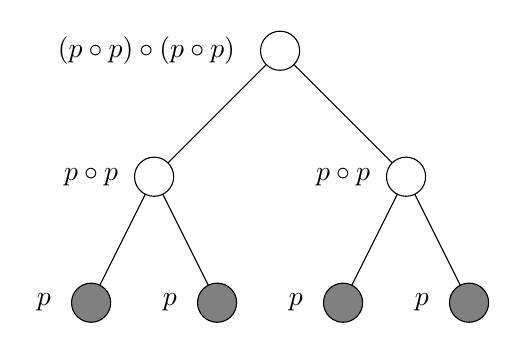
\begin{tikzpicture}[scale=0.8]

    \draw  (1,-1) -- (2,1);
    \draw  (3,-1) -- (2,1);
   \draw  (2,1) -- (4,3);
    \draw  (5,-1) -- (6,1);
    \draw  (7,-1) -- (6,1);
    \draw  (6,1) -- (4,3);

    \node[shape=circle, draw=black, fill = white, scale = 1.5]  at (4,3) {};
    \node[shape=circle, draw=black, fill = white, scale = 1.5]  at (2,1) {};
    \node[shape=circle, draw=black, fill = gray, scale = 1.5]  at (1,-1) {};
    \node[shape=circle, draw=black, fill = gray, scale = 1.5]  at (3,-1) {};
    \node[shape=circle, draw=black, fill = white, scale = 1.5]  at (6,1) {};
    \node[shape=circle, draw=black, fill = gray, scale = 1.5]  at (5,-1) {};
    \node[shape=circle, draw=black, fill = gray, scale = 1.5]  at (7,-1) {};

    \node at (1/4,-1) {$p$};
    \node at (9/4,-1) {$p$};
    \node at (17/4,-1) {$p$};
    \node at (25/4,-1) {$p$};
    \node at (1,1) {$p \circ p$};
    \node at (20/4,1) {$p \circ p$};
    \node at (8/4,3) {$(p\circ p) \circ (p \circ p)\;\;$};


\end{tikzpicture}
\end{subfigure}
\hspace{2 cm}
\begin{subfigure}

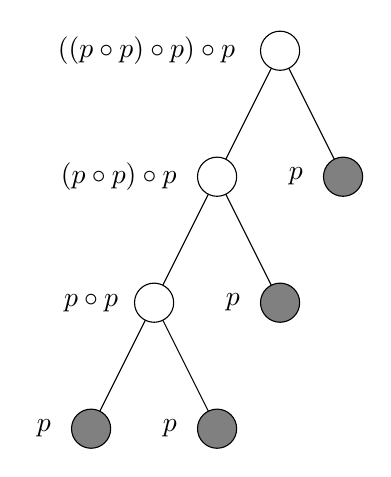
\begin{tikzpicture}[scale=0.8]

    \draw  (1,-3) -- (4,3);
    \draw  (3,-3) -- (2,-1);
    \draw  (4,-1) -- (3,1);
    \draw  (5,1) -- (4,3);

    \node[shape=circle, draw=black, fill = white, scale = 1.5]  at (3,1) {};
    \node[shape=circle, draw=black, fill = white, scale = 1.5]  at (2,-1) {};
    \node[shape=circle, draw=black, fill = gray, scale = 1.5]  at (1,-3) {};
    \node[shape=circle, draw=black, fill = gray, scale = 1.5]  at (3,-3) {};
    \node[shape=circle, draw=black, fill = gray, scale = 1.5]  at (4,-1) {};
    \node[shape=circle, draw=black, fill = white, scale = 1.5]  at (4,3) {};
    \node[shape=circle, draw=black, fill = gray, scale = 1.5]  at (5,1) {};

    \node at (1/4,-3) {$p$};
    \node at (9/4,-3) {$p$};
    \node at (1,-1) {$p \circ p$};
    \node at (13/4,-1) {$p$};
    \node at (17/4,1) {$ p$};
    \node at (6/4,1) {$(p\circ p) \circ p\;$};
    \node at (8/4,3) {$((p\circ p) \circ p)\circ p\;\;$};



\end{tikzpicture}
\end{subfigure}
\caption{Two possible trees $\g,\g'\in\G(4)$, and the corresponding distributions $C_{\gamma}(p) = (p\circ p) \circ (p \circ p)$ and $C_{\gamma'}(p) = ((p\circ p) \circ p)\circ p.$}\label{fig1}
\end{figure}



For example, if $k=3$, there are only two trees $\g,\g'\in\G(3)$, with $\a_3(\g)=\a_3(\g')=1/2$ and
\begin{align}\label{eq2}
C_{\gamma}(p)=(p \circ p)\circ p=p\circ(p \circ p)= C_{\gamma'}(p).
\end{align}
We refer to Figure~\ref{fig1} for two examples of $C_{\gamma}(p)$ for $\g\in\G(4)$.


Since each collision is of the form $q\circ q'$ for some $q,q'\in\cP(\O)$ and since by~\eqref{defconv1} one has
\begin{align}\label{lab:nons}
&p \circ q = \sum_{A\,\subset\,[n]}\bar\nu(A)\,p_A \otimes q_{A^c},
\end{align}
where $\bar\nu(A)= \frac12(\nu(A)+\nu(A^c))$, one can write the following expansion for the resulting measure at the root:
\begin{align}\label{eq5}
C_{\gamma}(p)= \sum_{\vec A\,\in\,\cV_n^{k-1}}\nu(\vec A) C^{\vec A}_{\gamma}(p),
\end{align}
where $\cV_n$ is the set of subsets of $[n]$, so that $\vec A\in \cV_n^{k-1}$ represents a pattern $\vec A=(A_1,\,\dots,\,A_{k-1})$,
\begin{equation}\label{eq:nua}
\nu(\vec A)= \prod_{i=1}^{k-1}\bar\nu(A_i)
\end{equation}
and $C^{\vec A}_{\gamma}(p)\in\cP(\O)$ is the distribution computed as follows. Each internal node $v_i$, $i=1,\,\dots\,,k-1$, in $\gamma$ (in some fixed order) is associated with the set $A_i$, and we attach the mark $A_i$ to the edge connecting $v_i$ to its left child and the mark $A_i^c$ to the edge connecting $v_i$ to its right child in $\gamma$. In this way we obtain a tree $\gamma$ with marks on all its edges. Let $d_i$ denote the depth of the $i^{\rm th}$ leaf of $\gamma$ (e.g.\ counting from the leftmost leaf), and consider $p_{V_i(\vec A)}$, the marginal of the measure $p$ on the subset
\begin{align}\label{eqa5}
V_i(\vec A):=\cap_{j=1}^{d_i} A^i_j,
\end{align}
where $A^i_1,\dots,A^i_{d_i}$ are the marks encountered along the edges of the unique path from the root to the $i^{\rm th}$ leaf. Then $ C^{\vec A}_{\gamma}(p)$ is given by
\begin{align}\label{eq6}
C^{\vec A}_{\gamma}(p) = p_{V_1(\vec A)}\otimes\cdots\otimes p_{V_k(\vec A)}.
\end{align}
Note that some of the $V_i(\vec A)$ may be empty. However, they form a partition of $[n]$, namely $V_i(\vec A)\cap V_j(\vec A)=\emptyset$ for $i\neq j$ and $\cup_{i=1}^kV_i(\vec A)=[n]$, which can be seen as the result of a fragmentation process
\[
[n]\to (A_1,A_1^c) \to (A_1\cap A_2,A_1\cap A_2^c,A_1^c)\to\cdots\to \left(V_1(\vec A),\cdots,V_k(\vec A)\right).
\]
As an example, in the case~\eqref{eq2} we have $\vec A=(A_1,A_2)$, and
\begin{align}
(p \circ p)\circ p = \sum_{A_1,\,A_2 \,\subset\,[n]}\bar\nu(A_1)\bar\nu(A_2)p_{A_1\,\cap\,A_2}\otimes p_{A_1\,\cap\,A_2^c} \otimes p_{A_1^c}.
\end{align}
The proof of~\eqref{eq00}-\eqref{eq5} can be easily done by induction, by splitting the tree $\g\in\G(k)$ into the left and right subtrees $\g_l,\g_r$ and using the relation~\eqref{eqreca}, see the proof of~\eqref{eq:idto} below for a closely related explicit computation.

In conclusion, from~\eqref{wildsums}, \eqref{eq00} and~\eqref{eq5} we obtain the following representation of the distribution $p_t$ as a convex combination of distributions $C^{\vec A}_{\gamma}(p)$:
\begin{align}\label{eq0}
p_t=\sum_{k=1}^{\infty}\b_t(k)\sum_{\g\,\in \,\Gamma(k)}\alpha_k(\g)\sum_{\vec A\,\in\, \cV_n^{k-1}}\nu(\vec A) \,C^{\vec A}_{\gamma}(p),
\end{align}
where $\b_t(k) := e^{-t}(1-e^{-t})^{k-1}$ is a probability on $\bbN$ for each $t\geq 0$, $ \alpha_k(\g)$ is a probability on $\G(k)$ for all $k$, and $\nu(\vec A)$ is a probability on $\cV_n^{k-1}$ for all $k$.

\begin{proof}
From~\eqref{eq0} we write
\begin{align}\label{eqb17}
S_t(p) - S_t(q) =\sum_{k=1}^\infty \b_t(k) s^{(k)},
\end{align}
where
\begin{align}\label{eqba17}
s^{(k)}=\sum_{\gamma\,\in\,\Gamma(k)}\alpha_k(\gamma)
\sum_{\vec A\,\in\,\cV_n^{k-1}}\nu(\vec A) \,\left[C^{\vec A}_{\gamma}(p)-C^{\vec A}_{\gamma}(q)\right]\,.
\end{align}
We introduce some further notation in order to handle more explicitly the difference of probability measures $C^{\vec A}_{\gamma}(p)-C^{\vec A}_{\gamma}(q)$. For any given $\g\in\G(k)$, and $\vec A\in \cV_n^{k-1}$, $\phi:\O\mapsto\bbR$, we may write
\begin{multline}\label{eqb28}
\scalar{C^{\vec A}_{\gamma}(p)-C^{\vec A}_{\gamma}(q)}{\phi}\\
 =\sum_{(x,y)\,\in\,\Omega^k\,\times\, \Omega^k}\mu(x,y) \sum_{z\,\in\,\Omega} \phi(z)\left(\ind\left(z=u(y,\vec A)\right)-\ind\left(z=u(x,\vec A)\right)
\right)
\end{multline}
where $x=(x^i,i=1,\,\dots,\,k)\in\O^k$ stands for the configurations sampled with $q^{\otimes k}$ over the leaves of $\g$, $y=(y^i,i=1,\,\dots,\,k)\in\O^k$ stands for the configurations sampled with $p^{\otimes k}$ over the leaves of $\g$, and $\mu(x,y)=\prod_{i=1}^k\mu_1(x^i,y^i)$ denotes a coupling of these two product measures, such that for every $i=1,\,\dots,\,k$, $\mu_1(x^i,y^i)$ is the optimal coupling of $(q,p)$:
\begin{align}\label{eq29}
\|p-q\|_{\tv} = \sum_{(x,y)\,\in\,\Omega^k\,\times\,\Omega^k}\mu(x,y) \ind\left(x^i\neq y^i\right)=\sum_{x^i,y^i\,\in\,\Omega}\mu_1\left(x^i,y^i\right) \ind\left(x^i\neq y^i\right).
\end{align}
The notation $u(x,\vec A)$ in~\eqref{eqb28} is defined as follows. Note that $x^i\in\O$ is a vector $x^i=(x^i_1,\,\dots,\,x^i_n)$, for every $i$, with $x^i_\ell\in\{0,\,\dots,\,q_\ell\}$, and write $x^i_A=(x^i_\ell)_{\ell\,\in\,A}$ for the content of $x^i$ on $A\subset[n]$. With this notation, given $x\in\Omega^k$ and $\vec A\in\cV_n^{k-1}$, $u(x,\vec A)\in\O$ is defined as the unique configuration such that
\[
u(x,\vec A)_{V_i(\vec A)} = x^i_{V_i(\vec A)}
\]
for every $i=1,\,\dots,\,k$. In words, for each $i\in[k]$, the content of the configuration $u(x,\vec A)$ on the set $V_i(\vec A)\subset V$ is taken from the configuration $x^i$ at the $i^{\rm th}$ leaf. The validity of~\eqref{eqb28} is thus a consequence of~\eqref{eq6}.

Let $\partial\g$ denote the set of leaves of $\g$. Notice that
\begin{gather*}
\ind(z=u(x,\vec A)) =
\prod_{i\,\in\,\partial \g}
\ind(z_{V_i(\vec A)}=x^i_{V_i(\vec A)})
\end{gather*}
Let $F=F(\vec A,\g)\subset \partial \g$ denote the set of leaves $i\in \partial \g$ such that $|V_i(\vec A)|> 1$, and write
\[
\ind(z=u(x,\vec A)) = w_F (x,z,\vec A) w_{F^c}(x,z,\vec A)\,,
\]
where for any $S\subset \partial \g$ we write
\begin{equation}\label{defwS}
w_S(x,z,\vec A) = \prod_{i\,\in\,S}
\ind(z_{V_i(\vec A)}=x^i_{V_i(\vec A)}).
\end{equation}
We write $X=(X^i)_{i=1,\,\dots,\,k}$ and $Y=(Y^i)_{i=1,\,\dots,\,k}$ for the random variables with distribution $q^{\otimes k}$ and $p^{\otimes k}$ respectively. Using the fact that $\mu$ is a product over the leaves, and the fact that $p,q$ have the same marginals, for fixed $z\in\O$ we have
\begin{align}\label{eq282a}
\begin{split}
\mu\left[w_{F^c} \left(X,z,\vec A\right)\right]&=\sum_{(x,y)}\mu(x,y) \prod_{i\,\in\, F^c}
\ind\left(z_{V_i(\vec A)}=x^i_{V_i(\vec A)}\right) \\
&= \sum_{(x,y)}\mu(x,y) \prod_{i\,\in\,F^c}
\ind\left(z_{V_i(\vec A)}=y^i_{V_i(\vec A)}\right) =
\mu\left[w_{F^c} (Y,z,\vec A)\right],
\end{split}
\end{align}
and
\begin{align}\label{eq282}
\begin{split}
\mu\left[w_{\partial \g}\left(Y,z,\vec A\right)\right]&=\sum_{(x,y)}\mu(x,y)
\ind\left(z=u(y,\vec A)\right)\\
&=\mu\left[w_{F^c} \left(X,z,\vec A\right)\right]\mu\left[w_F \left(Y,z,\vec A\right)\right].
\end{split}
\end{align}
With this notation we rewrite~\eqref{eqb28} as
\begin{multline}\label{eqbb28}
\left\langle C^{\vec A}_{\gamma}(p)-C^{\vec A}_{\gamma}(q),\phi\right\rangle\\
\begin{aligned}
&=
\sum_{z\,\in\,\Omega} \phi(z) \left[
\mu[w_{\partial \g}\left(Y,z,\vec A\right)] - \mu[w_{\partial \g}\left(X,z,\vec A\right)\right],
\\
&=
\sum_{z\,\in\,\Omega} \phi(z)
\mu\left[w_{F^c} \left(X,z,\vec A\right)\right]\,\mu\left[w_F \left(Y,z,\vec A\right)-w_F \left(X,z,\vec A\right)
\right].
\end{aligned}
\end{multline}
Note that $w_F (Y,z,\vec A)]\neq w_F (X,z,\vec A)$ implies that there exists $i\in F$ such that $X^i\neq Y^i$. Therefore, from~\eqref{eq29} we see that
\begin{multline}\label{eqbb2a8}
\sum_{z\,\in\,\Omega} \mu
\left[w_{F^c} \left(X,z,\vec A\right)\right]\,
\left|\mu
\left[w_F \left(Y,z,\vec A\right)-w_F \left(X,z,\vec A\right)
\right]\right|\\
\begin{aligned}
&\leq
\sum_{i\,\in\,F}\sum_{z\,\in\,\Omega} \mu\left[w_{F^c} \left(X,z,\vec A\right)\right]\,\mu\left[\left|w_F \left(Y,z,\vec A\right)-w_F \left(X,z,\vec A\right)\right|\ind\left(X^i\neq Y^i\right)
\right] \\
&\leq 2\sum_{i\,\in\,F}
\mu\left[X^i\neq Y^i
\right] = 2|F|\,\|p-q\|_\tv.
\end{aligned}
\end{multline}
Therefore, we have shown that~\eqref{eqba17} satisfies
\begin{align}\label{eq2aa86}
& \left|\left\langle s^{(k)},\phi\right\rangle\right|\leq 2\,\|\phi\|_\infty\,\|p-q\|_\tv \sum_{\gamma\,\in\,\Gamma(k)}\alpha_k(\gamma)
\sum_{\vec A\,\in\,\cV_n^{k-1}}\nu(\vec A)\,|F|.
\end{align}
To estimate~\eqref{eq2aa86}, let us call $\cA_{j}=\cA_j(\gamma)$ the set of $\vec A\in\cV_n^{k-1}$ such that $|V_j(\vec A)|\geq 2$, and let $\cA=\cup_{j=1}^k\cA_j$. If $\vec A\notin\cA$ then all sets $V_j(\vec A)$ are either empty or a single site and therefore $|F|=0$. Moreover, $|F|=\sum_{j=1}^k\ind(\cA_{j})$. Therefore we write
\begin{align}
\sum_{\vec A\,\in\,\cV_n^{k-1}}\nu(\vec A)\,|F|= \sum_{j=1}^k
\nu(\cA_j).
\end{align}
To estimate the probability $\nu(\cA_j)$, observe that the event $\cA_j$ implies that there exists $i_1<i_2\in[n]$ such that $\{i_1,i_2\} \in V_j(\vec A)$. Moreover, recalling~\eqref{eqa5},
\begin{align*}
\nu\left(\{i_1,i_2\} \in V_j(\vec A)\right)& = \nu\left(\{i_1,i_2\} \in \cap_{l=1}^{d_j} A^j_l\right) = \bar \nu\left(\{i_1,i_2\} \in A\right)^{d_j}
\leq \left(\frac{r(\nu)}{2}\right)^{d_j},
\end{align*}
where we use the fact that for any $i_1<i_2$, the probability under $\bar\nu$ that $\{i_1,i_2\} \in A$ is bounded by $r(\nu)/2$. Indeed, conditionally on not being separated the probability that both $i_1,i_2$ belong to $A$ under $\bar\nu$ is $1/2$ by symmetry. A union bound then shows that
\[
\nu(\cA_j)\leq \tfrac12\,n(n-1)\left(\frac{r(\nu)}{2}\right)^{d_j}.
\]
In conclusion, if we define
\begin{align}\label{eqomegagamma}
\o(\gamma):=\sum_{j=1}^k\left(\frac{r(\nu)}{2}\right)^{d_j},
\end{align}
we obtain, for all $k\in\bbN$,
\begin{align}\label{eq10}
& \left|\left\langle s^{(k)},\phi\right\rangle\right|\leq{n(n-1)}\,\|\phi\|_\infty\,\|p-q\|_\tv \sum_{\gamma\,\in\,\Gamma(k)}\alpha_k(\gamma)
\,\o(\g).
\end{align}
From~\cite[Lemma~1.4]{carlenwild}, one has, for all $\e>0$,
\begin{align}\label{carlenwildestimation}
\sum_{\gamma\,\in\,\Gamma(k)}\alpha_k(\gamma)\o(\gamma) \leq B_\e e^{-a_\e\log k}.
\end{align}
with $a_\e=(1-r(\nu))/(1+\e)$ and $B_\e=B_\e(r(\nu),\e)$. One could use this estimate to obtain an almost optimal decay rate $a_\e$. However, here we obtain the optimal exponential decay rate by computing the expectation of $\o(\g)$.

\begin{lemm}\label{lemma:omega}
For any $t\geq 0$,
\begin{equation}\label{lem:omega}
\sum_{k=1}^{\infty}\b_t(k)\sum_{\g\,\in \,\Gamma(k)}\alpha_k(\g)\,\o(\gamma) = e^{-(1-r(\nu))t}.
\end{equation}
\end{lemm}

Assuming the validity of~\eqref{lem:omega}, and using $\|\mu-\mu'\|_\tv = \tfrac12 \max_{f:\,\|f\|_\infty\leq 1} |\mu(f)-\mu'(f)|$, from~\eqref{eqb17} and~\eqref{eq10} we obtain
\begin{align}\label{eqabb17}
\|S_t(p) - S_t(q)\|_\tv
\leq \tfrac12\,n(n-1)\,\|p-q\|_\tv \,e^{-(1-r(\nu))t},
\end{align}
which concludes the proof of Theorem~\ref{contrlemma2}.

It remains to prove~\eqref{lem:omega}. For any $\g\in\cup_{k=1}^\infty\G(k)$, define $\bbP_t(\g) = \b_t(k)\alpha_k(\g)$, where $k$ is such that $\g\in\G(k)$. Notice that for any $\g\in\cup_{k=1}^\infty\G(k)$,
\begin{equation}\label{lem:omega1}
\bbP_t(\g) = \ind_{\g=\emptyset}\,e^{-t} + \ind_{\g\neq \emptyset}\int_0^t e^{-s}\bbP_{t-s}(\g_l)\bbP_{t-s}(\g_r)ds,
\end{equation}
where $\emptyset$ denotes the empty tree with one leaf (given by the root), while for $\g\neq \emptyset$ we write $\g_l,\g_r$ for the left and right subtrees. Indeed, for $\g=\emptyset$~\eqref{lem:omega1} is immediate, while for $\g\neq\emptyset$, supposing $\g\in\G(k)$, and recalling~\eqref{eqreca} one has
\begin{align*}
\bbP_{t}(\g) &= e^{-t}\left(1-e^{-t}\right)^{k-1}\a_k(\g) = e^{-t}\int_0^{t}e^{-(t-s)}\left(1-e^{-(t-s)}\right)^{k-2}(k-1)\a_k(\g)ds\\ &=
\int_0^t e^{-s}e^{-2(t-s)}\left(1-e^{-(t-s)}\right)^{k-2}\a_j(\g_l)\a_{k-j}(\g_r)ds =\int_0^t e^{-s} \bbP_{t-s}(\g_l)\bbP_{t-s}(\g_r)ds.
\end{align*}
To prove Lemma~\ref{lemma:omega}, note that the left hand side of~\eqref{lem:omega} is given by $\sum_\g \bbP_t(\g)\o(\g)$. Using~\eqref{lem:omega1} and $\o(\emptyset)=1$, we see that
\begin{align*}
\z(t):&=\sum_\g\bbP_{t}(\g)\o(\g) =e^{-t} +\frac{r(\nu)}2
\sum_{\g\neq\emptyset}\int_0^t e^{-s} \bbP_{t-s}(\g_l)\bbP_{t-s}(\g_r)(\o(\g_l)+\o(\g_r))ds\\
&=e^{-t} +r(\nu)
\sum_{\g}\int_0^t e^{-s} \bbP_{t-s}(\g)\o(\g)ds=e^{-t} +r(\nu)
\int_0^t e^{-s} \z(t-s)ds.
\end{align*}
Differentiating, and integrating by parts the resulting expression one finds $\dot\z(t) = -(1-r(\nu))\z(t)$. Since $\z(0)=1$ we obtain $\z(t)=e^{-(1-r(\nu))t}$, $t\geq 0$.
\end{proof}

\begin{thebibliography}{99}
\bibitem{Bertini_etal} Basile, G.; Benedetto, D.; Caglioti, E.; Bertini, L. Large deviations for a binary collision model: energy evaporation, Math. Eng., Volume 5 (2023) no. 1, 1, p. 12
\bibitem{barthe_et_al} Barthe, F.; Cordero-Erausquin, D.; Ledoux, M.; Maurey, B. Correlation and Brascamp–Lieb inequalities for Markov semigroups, Int. Math. Res. Not., Volume 2011 (2011) no. 10, pp. 2177-2216
\bibitem{bonetto2017entropy} Bonetto, F.; Geisinger, A.; Loss, M.; Ried, T. Entropy decay for the Kac evolution, Commun. Math. Phys., Volume 363 (2018) no. 3, pp. 847-875
\bibitem{BT} Bobkov, S. G.; Tetali, P. Modified logarithmic Sobolev inequalities in discrete settings, J. Theor. Probab., Volume 19 (2006) no. 2, pp. 289-336
\bibitem{asymm} Caputo, P.; Martinelli, F. Asymmetric diffusion and the energy gap above the 111 ground state of the quantum XXZ model, Commun. Math. Phys., Volume 226 (2002) no. 2, pp. 323-375
\bibitem{entprod} Caputo, P.; Sinclair, A. Entropy production in nonlinear recombination models, Bernoulli, Volume 24 (2018) no. 4B, pp. 3246-3282
\bibitem{carlenwild} Carlen, E. A.; Carvalho, M. C.; Gabetta, E. Central limit theorem for Maxwellian molecules and truncation of the Wild expansion, Commun. Pure Appl. Math., Volume 53 (2000) no. 3, pp. 370-397
\bibitem{entfound} Carlen, E. A.; Carvalho, M. C.; Le Roux, J.; Loss, M.; Villani, C. Entropy and chaos in the Kac model, Kinet. Relat. Models, Volume 3 (2010) no. 1, pp. 85-122
\bibitem{revchaos} Chaintron, L.-P.; Diez, A. Propagation of chaos: a review of models, methods and applications. I: Models and methods, Kinet. Relat. Models, Volume 15 (2022) no. 6, pp. 895-1015
\bibitem{cattiaux} Cattiaux, P.; Guillin, A.; Malrieu, F. Probabilistic approach for granular media equations in the non-uniformly convex case, Probab. Theory Relat. Fields, Volume 140 (2008) no. 1-2, pp. 19-40
\bibitem{Chung} Chung, K. L. A course in probability theory, Academic Press Inc., 2000
\bibitem{Virag} Csóka, E.; Harangi, V.; Virág, B. Entropy and expansion, Ann. Inst. Henri Poincaré, Probab. Stat., Volume 56 (2020) no. 4, pp. 2428-2444
\bibitem{elementary} Durmus, A.; Eberle, A.; Guillin, A.; Zimmer, R. An elementary approach to uniform in time propagation of chaos, Proc. Am. Math. Soc., Volume 148 (2020) no. 12, pp. 5387-5398
\bibitem{dolera_etal} Dolera, E.; Gabetta, E.; Regazzini, E. Reaching the best possible rate of convergence to equilibrium for solutions of Kac’s equation via central limit theorem, Ann. Appl. Probab., Volume 19 (2009) no. 1, pp. 186-209
\bibitem{DelMoralGuionnet} Del Moral, P.; Guionnet, A. On the stability of interacting processes with applications to filtering and genetic algorithms, Ann. Inst. Henri Poincaré, Probab. Stat., Volume 37 (2001) no. 2, pp. 155-194
\bibitem{miclo} Del Moral, P.; Miclo, L. Genealogies and increasing propagation of chaos for Feynman–Kac and genetic models, Ann. Appl. Probab., Volume 11 (2001) no. 4, pp. 1166-1198
\bibitem{DiacShash} Diaconis, P.; Shahshahani, M. Generating a random permutation with random transpositions, Z. Wahrscheinlichkeitstheor. Verw. Geb., Volume 57 (1981), pp. 159-179
\bibitem{DS} Diaconis, P.; Saloff-Coste, L. Logarithmic Sobolev inequalities for finite Markov chains, Ann. Appl. Probab., Volume 6 (1996) no. 3, pp. 695-750
\bibitem{erbar} Erbar, M.; Fathi, M.; Schlichting, A. Entropic curvature and convergence to equilibrium for mean-field dynamics on discrete spaces, ALEA, Lat. Am. J. Probab. Math. Stat., Volume 17 (2020) no. 1, pp. 445-471
\bibitem{einav2011villani} Einav, A. On Villani’s conjecture concerning entropy production for the Kac master equation, Kinet. Relat. Models, Volume 4 (2011) no. 2, pp. 479-497
\bibitem{Gei} Geiringer, H. On the probability theory of linkage in Mendelian heredity, Ann. Math. Stat., Volume 15 (1944), pp. 25-57
\bibitem{Goel} Goel, S. Modified logarithmic Sobolev inequalities for some models of random walk, Stochastic Processes Appl., Volume 114 (2004) no. 1, pp. 51-79
\bibitem{GQ} Gao, F.; Quastel, J. Exponential decay of entropy in the random transposition and Bernoulli–Laplace models, Ann. Appl. Probab., Volume 13 (2003) no. 4, pp. 1591-1600
\bibitem{grunbaumchaos} Grünbaum, F. A. Propagation of chaos for the Boltzmann equation, Arch. Ration. Mech. Anal., Volume 42 (1971), pp. 323-345
\bibitem{onkacschaos} Hauray, M.; Mischler, S. On Kac’s chaos and related problems, J. Funct. Anal., Volume 266 (2014) no. 10, pp. 6055-6157
\bibitem{KAC} Kac, M. Foundations of kinetic theory, Proceedings of the Third Berkeley Symposium on Mathematical Statistics and Probability, 1954–1955, vol. III, University of California Press (1956), pp. 171-197
\bibitem{lacker} Lacker, D. Hierarchies, entropy, and quantitative propagation of chaos for mean field diffusions, Probab. Math. Phys., Volume 4 (2023) no. 2, pp. 377-432
\bibitem{Lyubich} Lyubich, Y. I. Mathematical structures in population genetics, Biomathematics (Berlin), 22, Springer, 1992 (translated from the Russian by D. Vulis and A. Karpov. Edited by E. Akin)
\bibitem{Martinez} Martínez, S. A probabilistic analysis of a discrete-time evolution in recombination, Adv. Appl. Math., Volume 91 (2017), pp. 115-136
\bibitem{mckean1966speed} McKean, H. P. jun. Speed of approach to equilibrium for Kac’s caricature of a Maxwellian gas, Arch. Ration. Mech. Anal., Volume 21 (1966), pp. 343-367
\bibitem{mckean} McKean, H. P. jun. An exponential formula for solving Boltzmann’s equation for a Maxwellian gas, Comb. Theory, Volume 2 (1967), pp. 358-382
\bibitem{kacsprog} Mischler, S.; Mouhot, C. Kac’s program in kinetic theory, Invent. Math., Volume 193 (2013) no. 1, pp. 1-147
\bibitem{anewapp} Mischler, S.; Mouhot, C.; Wennberg, B. A new approach to quantitative propagation of chaos for drift, diffusion and jump processes, Probab. Theory Relat. Fields, Volume 161 (2015) no. 1-2, pp. 1-59
\bibitem{Nagylaki} Nagylaki, T. Introduction to theoretical population genetics, Biomathematics (Berlin), 21, Springer, 2013
\bibitem{Petrov} Petrov, V. V. Sums of independent random variables, Walter de Gruyter, 2022
\bibitem{review_discrete} Platkowski, T.; Illner, R. Discrete velocity models of the Boltzmann equation: a survey on the mathematical aspects of the theory, SIAM Rev., Volume 30 (1988) no. 2, pp. 213-255
\bibitem{Reza} Rezakhanlou, F. Propagation of chaos for particle systems associated with discrete Boltzmann equatio, Stochastic Processes Appl., Volume 64 (1996) no. 1, pp. 55-72
\bibitem{Sinetal2} Rabani, Y.; Rabinovich, Y.; Sinclair, A. A computational view of population genetics, Random Struct. Algorithms, Volume 12 (1998) no. 4, pp. 313-334
\bibitem{Sinetal} Rabinovich, Y.; Sinclair, A.; Wigderson, A. Quadratic dynamical systems, 33rd annual symposium on Foundations of computer science (FOCS)Proceedings, IEEE (1992), pp. 304-313
\bibitem{Baakeetal} Salamat, M.; Baake, M.; Baake, E. The general recombination equation in continuous time and its solution, Discrete Contin. Dyn. Syst., Volume 36 (2016) no. 1, pp. 63-95
\bibitem{sznitman} Sznitman, A.-S. Topics in propagation of chaos, Calcul des probabilités, Ec. d’Été, Saint-Flour/Fr (Lecture Notes in Mathematics), Volume 1464, Springer (1989), pp. 165-251
\bibitem{tanaka} Tanaka, H. Probabilistic treatment of the Boltzmann equation of Maxwellian molecules, Z. Wahrscheinlichkeitstheor. Verw. Geb., Volume 46 (1978), pp. 67-105
\bibitem{Vil} Villani, C. Cercignani’s conjecture is sometimes true and always almost true, Commun. Math. Phys., Volume 234 (2003) no. 3, pp. 455-490
\bibitem{Wild} Wild, E. On Boltzmann’s equation in the kinetic theory of gases, Proc. Camb. Philos. Soc., Volume 47 (1951) no. 3, pp. 602-609
\end{thebibliography}
\end{document}
